\documentclass{standalone}
\usepackage{tikz}
\usetikzlibrary{calc}
\begin{document}
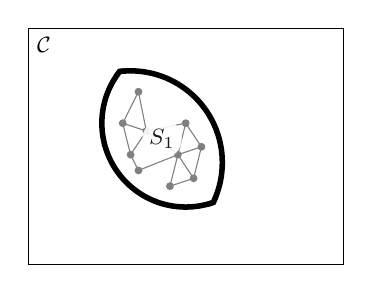
\begin{tikzpicture}

\tikzstyle{every node}=[font=\footnotesize]

\draw (0,0) rectangle (4.0,3.0);

\coordinate (a) at (2.0,1.8);
\coordinate (b) at (1.3,1.3);

\def\circlea{(a) circle (1.1)}
\def\circleb{(b) circle (1.2)}

% AnB
\begin{scope}
   \clip \circlea;
   \clip \circleb;
   \draw[line width=4pt] \circlea;
   \draw[line width=4pt] \circleb;
\end{scope}

% roadmap
\coordinate (v01) at ($ (a) + ( 0.0, 0.0) $);
\coordinate (v02) at ($ (a) + (-0.1,-0.4) $);
\coordinate (v03) at ($ (a) + ( 0.1,-0.7) $);
\coordinate (v04) at ($ (a) + (-0.2,-0.8) $);
\coordinate (v05) at ($ (a) + (-0.6,-0.6) $);
\coordinate (v06) at ($ (a) + (-0.7,-0.4) $);
\coordinate (v07) at ($ (a) + (-0.5,-0.1) $);
\coordinate (v08) at ($ (a) + ( 0.2,-0.3) $);
\coordinate (v09) at ($ (a) + (-0.8, 0.0) $);
\coordinate (v10) at ($ (a) + (-0.6, 0.4) $);
\node[circle,fill=black!50,inner sep=1.0] at (v01) {};
\node[circle,fill=black!50,inner sep=1.0] at (v02) {};
\node[circle,fill=black!50,inner sep=1.0] at (v03) {};
\node[circle,fill=black!50,inner sep=1.0] at (v04) {};
\node[circle,fill=black!50,inner sep=1.0] at (v05) {};
\node[circle,fill=black!50,inner sep=1.0] at (v06) {};
\node[circle,fill=black!50,inner sep=1.0] at (v07) {};
\node[circle,fill=black!50,inner sep=1.0] at (v08) {};
\node[circle,fill=black!50,inner sep=1.0] at (v09) {};
\node[circle,fill=black!50,inner sep=1.0] at (v10) {};
\draw[color=black!50]
   (v01) -- (v02) -- (v03) -- (v04) -- (v02) -- (v05) -- (v06)
   -- (v07) -- (v02) -- (v08);
\draw[color=black!50] (v03) -- (v08) -- (v01) -- (v07);
\draw[color=black!50] (v06) -- (v09) -- (v07) -- (v10) -- (v09);

\node at (0.2,2.8) {$\mathcal{C}$};

\node[circle,inner sep=1pt,fill=white,fill opacity=0.9]
  at (1.7,1.6) {$S_1$};

\end{tikzpicture}%
\end{document}
